%!TEX root = ../../pst-intro.tex

\chapter[Password Support Toolkit]{Password Support Toolkit}\label{chap:pct_intro}
The Password Coping Toolkit (PST) is a holistic approach to help users of any experience level manage their password portfolio of any size. Ideally, continuous usage of the PST enables and encourages users to 

there won't be a formula like ``if X then use strategy Y'' (magic wand strategy). Rather, one needs to give different aspects some thought. 

%%%%%%%%
% Questions
%%%%%%%
\section{Guiding Support Strategies}

\subsubsection{Roadmap}
\begin{tabular}{p{14cm}l}
	What is the desired outcome? & Outcome \\
	How difficult is it to achieve and why? & Difficulty \\
	How big would the impact be? & Impact \\
	How important is it to achieve this outcome? & Importance
\end{tabular}

\subsubsection{Strategy}
\begin{tabular}{p{14cm}l}
	What exactly is the strategy based on? & Foundation\\
	Why is it expected to work? & Support\\
	What stage(s) in the password life cycle does it target? & Stage \\
	What is the specific context? & Context \\
	Are there other ways to achieve the same effect? & Alternatives \\
	Who is the target user group? & User Group\\
	How does the strategy relate to other frameworks? & Relationships\\
	Is it a one-off effort or continuous support? & Time-Scale \\
\end{tabular}

\subsubsection{Prerequisites}
\begin{tabular}{p{14cm}l}
	What are the dimensions of user needs in this context? & Needs \\
	How can the needs be met by the strategy? & Match \\
	What are the characteristics of the strategy? & Characteristics\\
	What are the minimum abilities that the user needs to have? & Abilities\\
\end{tabular}

\subsubsection{Risks}
\begin{tabular}{p{14cm}l}
	Will users get habituated to the strategy and is this good or bad? & Habituation\\
	How would the strategy interfere with other solutions? & Interference\\
	Does the strategy require too much effort from the users? & Effort\\
\end{tabular}

\subsubsection{Evaluation}
\begin{tabular}{p{14cm}l}
	How is the strategy going to be evaluated? & Method\\
	Is it possible to triangulate methods? & Triangulation\\
	What are the metrics to track impact? & Metrics	
\end{tabular}





\todo{Decide on a final name of the tookit.}
extension to persuasive authentication framework. 

\begin{enumerate}
\item[a)] improve their strategies
\item[b)] strengthen the passwords
\item[c)] boost memorability of passwords
\end{enumerate}

All this leads to an improvement of user experience as both pragmatic and hedonic qualities are maximized. 



\begin{figure}
	\centering
	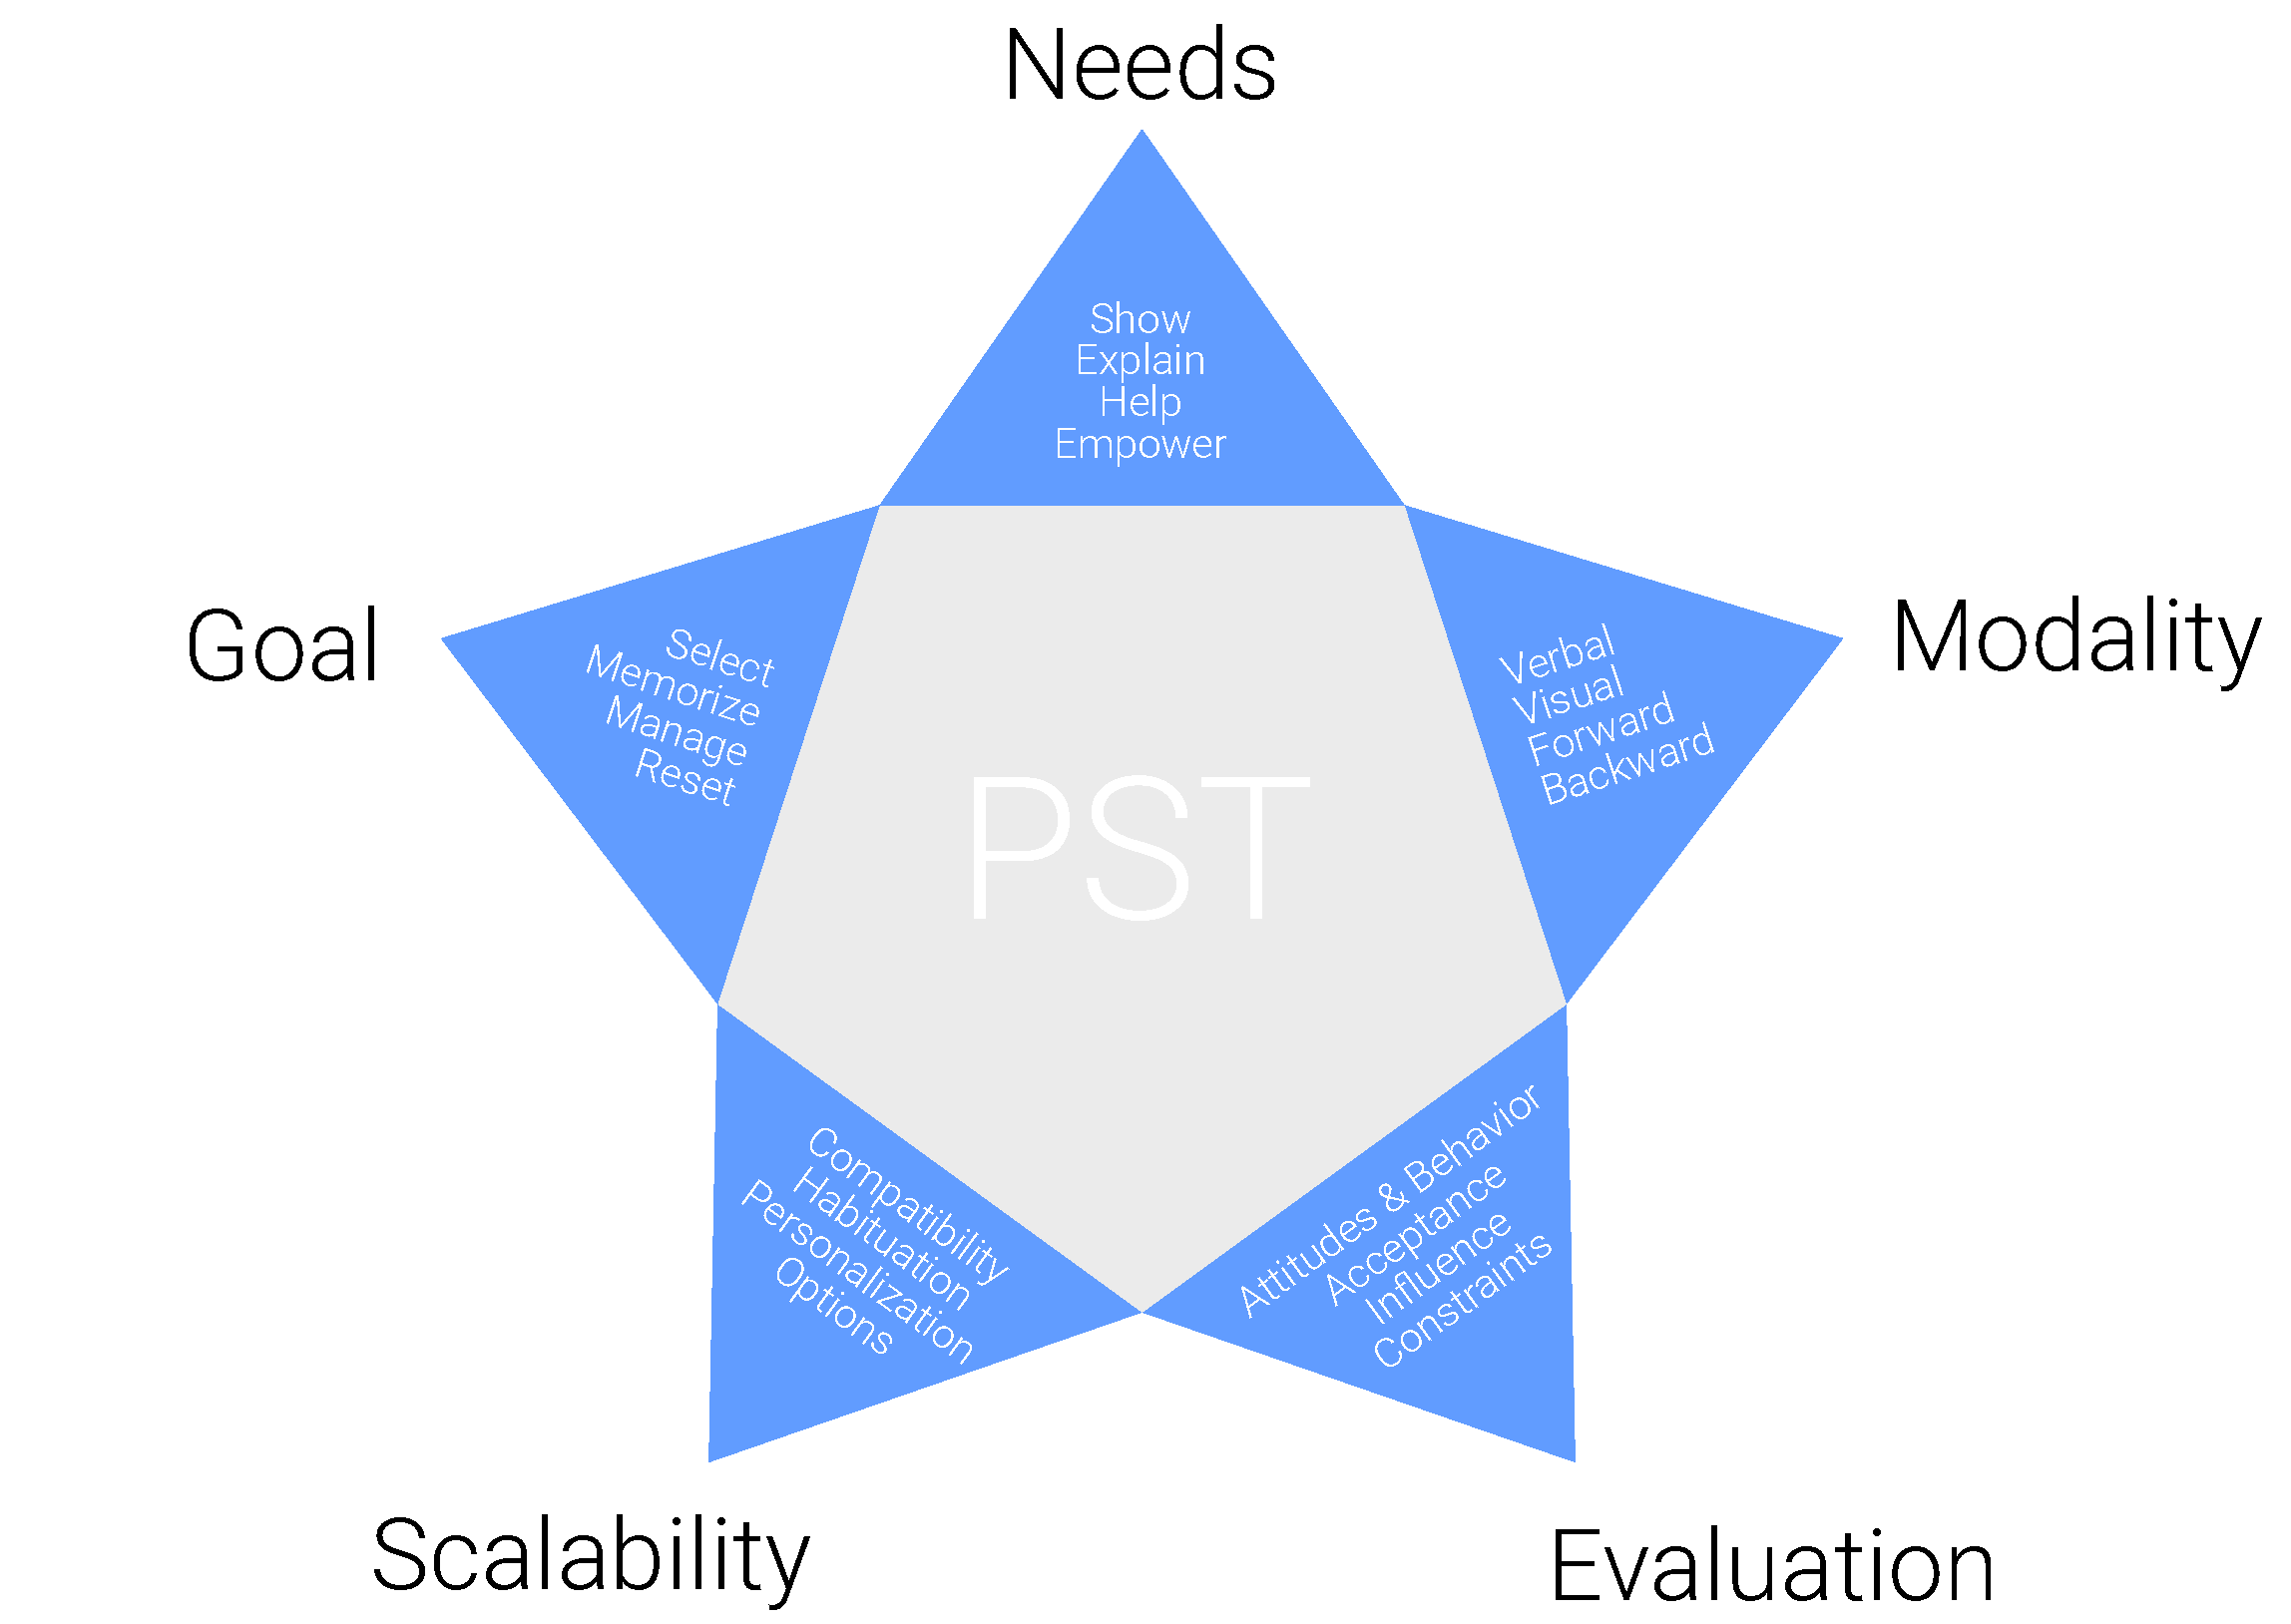
\includegraphics[width=0.8\linewidth]{figures/pst/PST-Star}
	\caption{\label{fig:pst:pst-star} Password Support Toolkit for Persuasive Strategies}
\end{figure}


\section{Respecting Privacy Concerns}
To make sure users can fully benefit from the power of the PCT, it is required that no information about the user's behavior travels through the web, i.e. to remote servers. Such knowledge would deeply compromise protection against foreign access. Attackers would intensify attacks on the stored behavioral data that would allow them to reverse engineer credentials. This has to be avoided at all costs. Consequently, the calculations need to take place on the client-side. With increasing computational power even for consumer electronic devices this does not seem to be a tough restriction. 

\section{Adapting to Existing Strategies}
As discussed in Chapter \ref{sec:password_selection}, each individual user handles password selection and memorization differently, even though patterns occur. 

The most prevalent factors for password selection are:
\begin{itemize}
\item Account Value
\item Memorability
\item \textbf{Perceived Strength}. As we have seen, people's perception of strength has changed, so as to speak ``they were enlightened''. Everyday practice has taught users that difficult passwords are good, but everybody thinks that they seem hard to do. The PCT allows to shift this perception. 
\end{itemize}

The PCT lets the user know, that their strategy is legitimate. It acknowledges them and does not want to change them.  Even password re-use can be beneficial.

The PCT addresses password strategies, by learning them through both active involvement and observation. 


\subsection{Learning Account Values}
The PCT adjusts nudges and persuasion to the users' perceived value of a password. 

\subsubsection{Measuring Password Value}
Users often fail to assess the value of passwords correctly as we have seen in (@TODO REF SEC). 

\subsection{Respect Context Factors beyond Account Value}
Groß \etal argued that cognitive depletion has a notable impact on the strength of passwords \cite{Gross2016EffectCognitiveEffort}. They proposed including a remark like ``Only set a new password when you feel fresh and awake'' in password advice. This kind of remark fits best in a password reset task. 


\section{Composition Policy Fulfillment}
Apple already has something like this (generate ``FIPS compatible'' password), but it doesn't speak the user's language nor does it explain what this is and when using it is necessary. Our idea is to take the user out of the loop and not burden them with such decisions when they feel the need to generate a password. 

\section{Supporting Memorization}
After the users picked their password, be it completely independently or with aid by the PCT, they are now facing the critical stage of memorizing it. In case they simply re-used or modified an old password, this phase is very short. They might write down which of their ready-made credentials they utilized. This is necessary and helpful if the account value is not clear or might change in the future. 

However, in case the PCT manage to persuade a user towards are slightly different option than they would have chosen without it, memorization is extremely important. As such, the PCT provides means to support this process in @TODO ways:
\begin{itemize}
\item training. 
\item \textbf{Storing}. The password is stored and can be retrieved from a local database. 
\end{itemize}

generate memorable passwords when appropriate. 

\section{Hedonic Qualities}
Hedonic UX qualities are often overlooked. The design and incorporates them from the very beginning. 

\section{Nudging Where Appropriate}
our results so far showed mixed results about successful nudges. 


Conclusions: Most mitigations seem to fit better into the scenario when the user resets their password. This has a couple of advantages:
\begin{itemize}
	\item The system already knows the user. This can be either a webservice provider or a password manager. So, it can tailor the experience and take a wide range of context factors into account. 
\end{itemize}


\section{Further Considerations}

\textbf{Persuasion is always opinionated}. The choice architect has a target behavior in mind, and it is an essential feature of persuasion opposed to manipulation that this target is in the user's own interest, and they can freely choose to act differently. 


\section{Evaluation Methods}
Rewind the methods that we used and show when to use which for evaluating different dimensions in persuasive design for passwords. 


